% IF YOU CAN SEE THIS GO CONTRIBUTE >:(

\documentclass[letterpaper, 8pt]{extarticle}
\usepackage{amssymb,amsmath,amsthm,amsfonts}
\usepackage{multicol,multirow}
\usepackage{calc}
\usepackage{ifthen}
\usepackage[landscape]{geometry}
\usepackage[colorlinks=true,citecolor=blue,linkcolor=blue]{hyperref}

\usepackage{booktabs}
\usepackage{ulem}
\usepackage{enumitem}
\usepackage{tabulary}
\usepackage{graphicx}
\usepackage{siunitx}
\usepackage{tikz}
\usepackage{derivative}
\usepackage{svg}
\usepackage{listings}
\usepackage{setspace}
\usepackage{listings}
\usepackage{xcolor}
\usepackage{courier}
\usepackage{syntax}
\usepackage{mathpartir}

% minimal line spacing
% \setstretch{0.1}

% set borders (experimentally determined to minimize cutoff and maximize space on school printers)
\geometry{top=.25in,left=.25in,right=.25in,bottom=.35in}

% make figures work better in multicol
\newenvironment{Figure}
{\par\medskip\noindent\minipage}
{\endminipage\par\medskip}

\pagestyle{empty} % clear page

% rewrite section commands to be smaller
\makeatletter
\renewcommand{\section}{\@startsection{section}{1}{0mm}%
                                {-1explus -.5ex minus -.2ex}%
                                {0.5ex plus .2ex}%x
                                {\normalfont\normalsize\bfseries}}
\renewcommand{\subsection}{\@startsection{subsection}{2}{0mm}%
                                {-1explus -.5ex minus -.2ex}%
                                {0.5ex plus .2ex}%
                                {\normalfont\small\bfseries}}
\renewcommand{\subsubsection}{\@startsection{subsubsection}{3}{0mm}%
                                {-1ex plus -.5ex minus -.2ex}%
                                {1ex plus .2ex}%
                                {\normalfont\tiny\bfseries}}
\makeatother
\setcounter{secnumdepth}{0} % disable section numbering


% disable indenting
\setlength{\parindent}{0pt}
\setlength{\parskip}{0pt plus 0.5ex}

% Custom siunitx defs
\DeclareSIUnit\noop{\relax}
\NewDocumentCommand\prefixvalue{m}{%
\qty[prefix-mode=extract-exponent,print-unity-mantissa=false]{1}{#1\noop}
}

% Shorthand definitions
\newcommand{\To}{\Rightarrow}
\newcommand{\ttt}{\texttt}
\newcommand{\ra}{\rightarrow}

% condense itemize & enumerate
\let\olditemize=\itemize \let\endolditemize=\enditemize \renewenvironment{itemize}{\olditemize \itemsep0em}{\endolditemize}
\let\oldenumerate=\enumerate \let\endoldenumerate=\endenumerate \renewenvironment{enumerate}{\oldenumerate \itemsep0em}{\endoldenumerate}
\setlist[itemize]{noitemsep, topsep=0pt, leftmargin=*}
\setlist[enumerate]{noitemsep, topsep=0pt, leftmargin=*}

\title{3GC3}

\begin{document}
\raggedright
\tiny

% make listings look nicer
\lstset{
    tabsize = 2, %% set tab space width
    showstringspaces = false, %% prevent space marking in strings, string is defined as the text that is generally printed directly to the console
    basicstyle = \tiny\ttfamily, %% set listing font and size
    breaklines = true, %% enable line breaking
    numberstyle = \tiny,
    postbreak = \mbox{\textcolor{red}{\(\hookrightarrow\)}\space}
}

\begin{center}
    {\textbf{3GC3 Midterm - Solaris-3 Edition}} \\
\end{center}
% set column spacing rules
\setlength{\premulticols}{1pt}
\setlength{\postmulticols}{1pt}
\setlength{\multicolsep}{1pt}
\setlength{\columnsep}{2pt}
\begin{multicols*}{4}

\section{Graphics Pipeline}

\section{Transformations \& Coordinate Systems}
\textbf{Linear Transformation}:
\(
f(\begin{bmatrix}
    x \\ y
\end{bmatrix})
= \begin{bmatrix}
    a_{11} & a_{12} \\
    a_{21} & a_{22}
\end{bmatrix}
\begin{bmatrix}
    x \\ y
\end{bmatrix}
=
\begin{bmatrix}
    a_{11} x + a_{12} y \\
    a_{21} x + a_{22} y
\end{bmatrix}
\)
satisfies: \(
f(\mathbf{u} + \mathbf{v})
= f(\mathbf{u}) + f(\mathbf{v})
\)
and
\(
f(c\mathbf{u}) = cf(\mathbf{u})
\)

In other words, origin is unchanged, straight lines remain straight lines.

\textbf{Affine Transformation}
Straight lines remain lines.

\textbf{2D Rotations}
\(
f(p)
= x \begin{bmatrix}
    \cos \theta \\ \sin \theta
\end{bmatrix}
+ y \begin{bmatrix}
    -\sin \theta \\ \cos \theta
\end{bmatrix}
= \begin{bmatrix}
    \cos \theta & - \sin \theta \\
    \sin \theta &   \cos \theta
\end{bmatrix}
\begin{bmatrix}
    x \\ y
\end{bmatrix}
\)

\textbf{3D Rotations}
For a generic 3D rotation:
\(
R =
\begin{bmatrix}
    ax & bx & cx \\
    ay & by & cy \\
    az & bz & cz
\end{bmatrix}
\)
Where the \(a*\) column is the coordinates of the object's \(x'\) vector,
the \(b*\) column is the \(y'\) vector,
and the \(c*\) column is the \(z'\) vector:
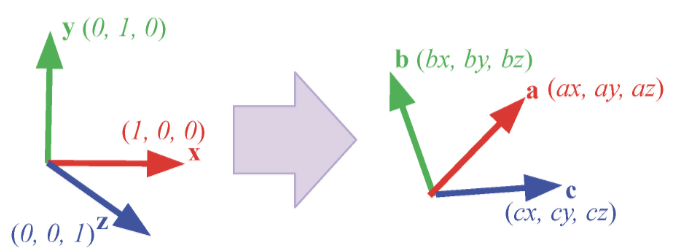
\includegraphics[width=\linewidth]{3d-rotation.png}

\textbf{2D Reflection}
Reflect X:\@
\(
\begin{bmatrix} -1 & 0 \\ 0 & 1 \end{bmatrix}
\)
Reflect Y:\@
\(
\begin{bmatrix} 1 & 0 \\ 0 & -1 \end{bmatrix}
\)

\textbf{3D Scaling}
\(
\begin{bmatrix}
    s_x & 0 & 0 \\
    0 & s_y & 0 \\
    0 & 0 & s_z
\end{bmatrix}
\begin{bmatrix}
    x \\ y \\ z
\end{bmatrix}
=
\begin{bmatrix}
    s_x x \\ s_y y \\ s_z z
\end{bmatrix}
\)

\textbf{2D Shear Matrix}
Horizontal shear:
\(
\begin{bmatrix}
    1 & s_x \\
    0 & 1
\end{bmatrix}
\)
Vertical shear:
\(
\begin{bmatrix}
    1 & 0 \\
    s_y & 1
\end{bmatrix}
\)


\section{Math}

\textbf{Dot Product}:
\(
\mathbf{a} \cdot \mathbf{b}
= x_a x_b + y_a y_b + z_a z_b
= ||\mathbf{a}|| ||\mathbf{b}|| \cos \phi
\)

\textbf{Cross Product}:
\(
\mathbf{a} \times \mathbf{b}
= (y_a z_b - z_a y_b, z_a x_b - x_a z_b, x_a y_b - y_a x_b)
= ||\mathbf{a}|| ||\mathbf{b}|| \sin(\theta) \mathbf{n}
\)

\textbf{Interpolation}:
\(t\) is how far along the line \(p_t\) is from \(p_0\) to \(p_1\) as a percentage between 0 and 1.
\(
t = (x_t - x_0) / (x_1 - x_0)
\text{ or }
t = (y_t - y_0) / (y_1 - y_0)
\)
\(
v_t = (1-t) v_0 + t v_1
\)

\textbf{Barycentric Interpolation}:
\(
\alpha = A_a / A \quad
\beta = A_b / A \quad
\gamma = A_c / A \quad
s.t.\ \alpha + \beta + \gamma = 1
\)

Now,
\(
\mathbf{p}(\alpha, \beta, \gamma)
= \alpha \mathbf{a} + \beta \mathbf{b} + \gamma \mathbf{c}
\)

\section{Camera}

\section{Rasterization}

\section{Fragment Shader}

\section{Depth Testing}

\section{Gransparency \& Blending}

\section{Other}

\end{multicols*}

\end{document}
